\chapter{Rule-based systems}
\label{cha:rules}

Rule-based systems---or RBS for short---provide means to operate on and store some data in a knowledge base. This data is often called knowledge or information and is stored in form of \emph{rules} and \emph{facts}.

The plot of accumulated article and citation counts in \cref{fig:scholar-rule-based} was obtained after processing 10167 articles on the subject. Again, like in \cref{cha:recommenders}, the resulting curves are S-shaped, an indicator of the fact, that thorough research had already been conducted on the matter and relatively little is being published nowadays.

\begin{figure}
	\centering
	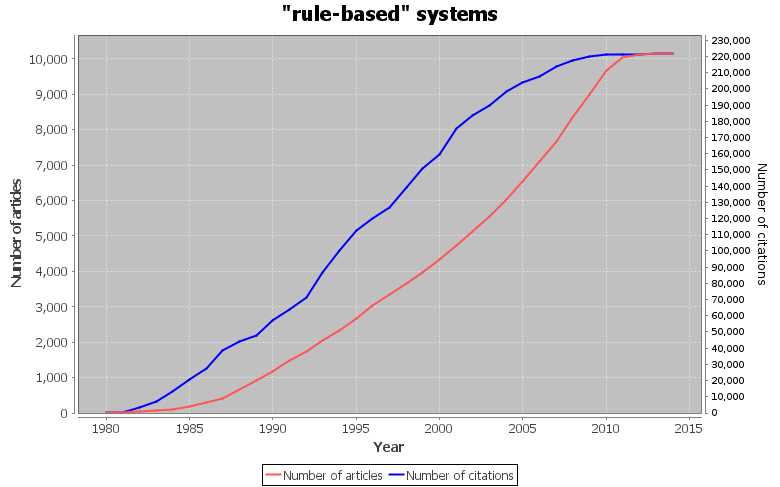
\includegraphics[width=0.95\textwidth]{scholar-rule-based}
	\caption{Google Scholar and Microsoft Academic Search accumulated trending for ``rule-based systems'' query \cite{Rus:scholar-trends}.}
	\label{fig:scholar-rule-based}
\end{figure}

Although the proposed solution is not a rule-based system per se, it uses a simple rule-based component (see more about that in \cref{sec:architecture}).

The \emph{rules} mentioned earlier are most often written in the form of \texttt{IF~a~THEN~b}, where these \texttt{a} and \texttt{b} components may represent almost anything \cite{Smith:krr}. In particular, the \texttt{b} part could be an assertion of some other information (that is adding the new information to the knowledge base). The \emph{facts} are just simple facts.

In very simple terms, an example of a fact could be \texttt{Ann is a human}. If it had also some corresponding rule defined, say, \texttt{IF \underline{X} is a human, THEN \underline{X} is going to die}, it would be possible to automatically infer and assert the fact that \texttt{Ann is going to die}. Similarly, facts can be retracted (or deleted) from the knowledge base.

In thinking about how this approach is different from regular programming--- ``regular'' as in ``imperative'', for functional programming languages show some similarities---it is really important to notice, that---in their purest form, in theory---rule-based systems do not impose any order in which rules are going to be executed. At least, that is the suggested mindset when defining rules of a particular RB system.

Usually, a rule-based systems is composed of at least three main components (the first three on the list below).

\begin{itemize}
	\item A rule base (knowledge base) described above, consisting of a set of rules (and, possibly, predefined facts).
	\item A reasoning engine (also called inference engine). It usually works in three phases. \begin{enumerate}
		\item In the first step, all rules are matched against the working memory (containing all previously asserted facts) and these with their left side (\texttt{IF a}) satisfied are chosen. From these rules, the \emph{conflict set} is built. If the set is empty, execution halts until there are more/less facts known, and after some are asserted/retracted, it begins again at step one.
		\item Then, in the second step, only one rule is chosen from the conflict set. There are different strategies for resolving this conflict (``which rule to run first'').
		\item This rule is executed. Its right side, \texttt{THEN b} is run. The execution might change the contents of working memory. The whole process is now looped and starts again at the first step (with possibly modified working memory).
	\end{enumerate}
	\item The inference engine also has to be equipped with so called \emph{working memory}, in which the current mutable state of the system is residing. The engine will be modifying this memory.
	\item Another very common part would of course be some user interface to interact with the system (ask questions, modify the knowledge, rules etc.).
\end{itemize}

Some other differences from regular programming---apart from no obvious order of execution---can be also thought of as advantages of this approach. They are listed below.

\begin{itemize}
	\item Arguably, the most important one is lower knowledge acquisition and maintenance cost. In regular computer systems, to change or define their rules of functioning, a programmer needs to be used, apart from an expert in given field. In case of RBS, the rules are usually notated/presented in a form that is capable of being understood by a field expert. They can delete, modify and define new rules without programmer's help.
	\item It is possible for the system to explain its decisions (e.g. using backtracking). It is incredibly important for simplification of verifying the correctness of its decisions. As the knowledge is contained explicitly in the rules, it is usually not hard to obtain a chain of reasoning and present it to the user. (That also is the intelligibility mentioned in \cref{sec:context-aware}.)
\end{itemize}

Inference engines may use two modes of operation: forward and backward chaining. The sample engine described above is using forward chaining. This method can also be thought of as incrementally applying \emph{modus ponens}:

\begin{equation}
	((P \to Q) \land P) \to Q
	\label{eq:modus-ponens}
\end{equation}

\Cref{eq:modus-ponens} claims that whenever we have a rule, $P \to Q$ and know that a fact sitting on its left hand side is true, $P$, we also know that $Q$ must be true. Iteratively applying this law of logic to the working memory and the defined rules is the core of forward chaining.

In backward chaining, there's a goal/question set forth by the user of the system. Then, the system, working backwards, is looking for rules with right hand side satisfying the goal (or those satisfying left hand sides from previous links in the chain of reasoning). If it happens so that all left hand sides are satisfied, the goal/question is true. Backward chaining systems usually employ depth-first strategy for traversing the knowledge graph \cite{chein2008graph}. One notable example of a language implementing backward chaining and DFS is Prolog.

Hayes-Roth et al. claim in \cite{hayes1984building}, that one advantage of forward-- over backward chaining systems is that the first is data-driven, and not by the goal. What that means is that arrival of new data (facts) can trigger new actions, the inference and the system on the whole are naturally more reactive.

The most obvious and widely-discussed use case for a rule-based system is an \emph{expert system}, one that is able to successfully emulate the decision making process of a human expert. Expert systems were the first truly successful achievement in the artificial intelligence software field \cite{russell1995artificial}.

Hayes-Roth in his already mentioned book, \cite{hayes1984building}, divides expert systems into ten distinct categories: interpretation, prediction, diagnosis, design, planning, monitoring, debugging, repair, instruction and control (tidbit: a system from the ``control'' group implemented in CLIPS, a rule-based language by NASA, was until recently used for Space Shuttle Mission Control \cite{rasmussen1990inco}). All this shows the vast applicability of rule-based systems.

\section{HeaRTDroid}

One example of rule-based systems that might be of particular interest for this project is the HeaRTDroid project \cite{heartdroid}. As the last part of the name suggests, it is meant to be run on mobile devices controlled by the Android system. Because of that, it was the first technology to turn to, as the proposed solution is meant to run on mobile devices.

As its developers claim in \cite{heartdroid}, the inference engine works with rules defined using XTT2 representation. XTT (Extended Tabular Trees), the predecessor of XTT2, was introduced by Nalepa in \cite{nalepa2004new}. Its ideas are based on ALSV---or Attributive Logic with Set Values---a concept described by Ligęza (its author) in \cite{ligeza2006rule}, sometimes referred to as ALSV(FD)---Attributive Logic with Set Values over Finite Domain---in the literature.

In ALSV(FD), the basic idea is that an attribute of a rule, say, \texttt{person in the room} needs not be satisfied with only one defined value, e.g. \texttt{Alice} (``taking an \emph{atomic} value''), but can also ``take a set of values'', i.e. be defined to be satisfiable with any of the values of some set, eg. \texttt{\{Alice, Bob, Cécile\}}.

Nalepa states in \cite{nalepa2008xtt2}:

\begin{quotation}
	``XTT is a knowledge representation and design formalism for \emph{rules}. It serves both as a \emph{logical} and \emph{algebraic} specification of rules \elide.
	
	In contrast to \elide a \emph{flat} (single-level) set of rules (e.g. using the Rete-based inference engines), XTT introduces an explicit \emph{structure} \elide: \emph{tables}, used to represent groups of rules working in the same context (having similar structure of preconditions), and \emph{intertable links}, used to provide explicit specification of inference control, \elide, that allow for decision-tree like structure.
	
	Each table is composed of its scheme \elide definition \elide, and
	the rules defined by the operators and values \elide.
	The method is used during the phase of the logical design of the rulebase. \elide
	
	XTT is a formal method based on an expressive logical calculus called Attributive Logic (or Attribute Logic).''
\end{quotation}

Interesting as these concepts seem, they are also surprisingly unknown outside of their authors. This claim is based on Google Scholar results for queries about subsequently: \texttt{"xtt2"~+rules}\footnote{\url{https://scholar.google.com/scholar?q="xtt2"+\%2Brules}} (17 of the 143 publications found were unrelated to the authors) and \texttt{"Attributive Logic with Set Values"}\footnote{\url{https://scholar.google.com/scholar?q="Attributive+Logic+with+Set+Values"}} (3 unrelated of the 26 results) and \texttt{"ALSV(FD)"}\footnote{\url{https://scholar.google.com/scholar?q="ALSV\%28FD\%29"}} (2 unrelated of the 55).
